\documentclass[conference]{IEEEtran}
\usepackage{graphicx}
\usepackage{amsmath}
\usepackage{booktabs}
\usepackage[hidelinks]{hyperref}

\begin{document}

\title{A State-of-Health-Aware Framework for Synthetic Inertia Delivery\\in Solar and Wind-Integrated Grids}

\author{\IEEEauthorblockN{Akshat Sharma, Rudraksh Sharma, Krishna Gahlod, Suryangshu Das, Sai Charan}
\IEEEauthorblockA{CM617, IIT Bombay}}

\maketitle

\begin{abstract}
Synthetic inertia studies usually assume a battery that always delivers its rated power. We model how ageing limits that power in a system powered only by solar or only by wind, with a grid-forming battery as the only source of inertia. A random forest trained on Sandia cycling data predicts state of health (SoH) from operating conditions, and a resistance model fitted on Severson LFP cells turns SoH into deliverable power. With real 2025 solar and wind data for Kutch, Gujarat, the aged battery responds like a fresh one until it reaches its power limit. LFP never does in 15 years; NMC and NCA miss up to 1.2\% of trip events. SoH-aware operation removes every failure at almost no cost.
\end{abstract}

\section{Introduction}
Solar and wind plants connect through inverters and add no rotating mass, so system inertia shrinks as they grow. Grid-forming (GFM) batteries can emulate inertia, but existing formulations assume an undegraded battery, although rising internal resistance and capacity fade lower the power an aged battery can deliver. This work links battery ageing to the synthetic inertia a GFM battery can actually provide in solar-only and wind-only systems, compares LFP, NMC and NCA chemistries, and tests whether chemistry choice, reserve sizing or SoH-aware operation keeps the response adequate over the battery's life.

\section{Data and Methods}
\subsection{SoH model (Model 1)}
We use the Sandia cycling data set \cite{preger2020}: 85 commercial 18650 cells (LFP, NMC, NCA) cycled under 33 conditions (15 to 35\,\textdegree C, three SOC windows, 0.5 to 3C discharge). From the periodic capacity checks we obtain 566 SoH labels. A random forest predicts SoH from chemistry, temperature, depth of discharge (DoD), discharge rate and equivalent full cycles. Capacity, voltage and time-based inputs were excluded to avoid leaking the answer. Tested on cells never seen in training it reaches $R^2 = 0.87$ (RMSE 0.023), and on whole test conditions never seen it reaches $R^2 = 0.81$ (RMSE 0.029), against 0.55 and 0.50 for a straight line per chemistry.

\subsection{Resistance and power model (Model 2)}
Sandia does not report resistance, so the link from SoH to resistance is learned from 124 LFP cells of Severson \emph{et al.} \cite{severson2019}, split by cell (41 training, 43 test). On the test cells the common linear formula $R/R_0 = 1 + \alpha(1-\mathrm{SoH})$ reaches $R^2 = 0.74$; its slope varies widely from cell to cell ($\alpha = 0.70 \pm 0.29$) and it misses the faster rise near end of life. A quadratic fit,
\begin{equation}
R/R_0 = 1 + 0.393\,x + 3.02\,x^2, \qquad x = 1 - \mathrm{SoH},
\end{equation}
reaches 0.78, and a random forest on SoH alone 0.79. A forest that also uses cycle number and temperature reaches 0.85, but those inputs describe Severson's fast-charging tests rather than grid duty, and a forest cannot be used smoothly outside its data. We therefore use the quadratic curve. With a fixed voltage window the deliverable power scales as $P_{\max} \propto 1/R$; at SoH 0.82 the battery keeps 86\% of its fresh power.

\subsection{Operating scenario}
Hourly 2025 output of a solar plant and of a wind farm (Vestas V90 2\,MW turbines) at Kutch, Gujarat (23.25\,N, 69.67\,E), and the site air temperature, come from Renewables.ninja \cite{staffell2016}. A 100\,MW plant is paired with a 25\,MW / 50\,MWh GFM battery (90\% round-trip efficiency), which is the only source of inertia. The battery keeps a reserve of 12.5\,MW and the 10 to 30\% charge band for frequency support, and uses the rest to smooth the plant towards its 24-hour mean. Load equals plant plus battery output. This duty gives 208 (solar) and 214 (wind) equivalent full cycles per year at 60\% DoD and 28.0 / 26.5\,\textdegree C, which Model 1 turns into SoH per year and Model 2 into the power ceiling.

Each year is replayed with the aged battery in two ways. \emph{SoH-unaware}: the operator keeps using 12.5\,MW for smoothing, so ageing eats into the reserve. \emph{SoH-aware}: smoothing is capped at (power ceiling $-$ 12.5\,MW) and enough charge is kept to hold the reserve for 15 minutes. In every hour the plant produces (4,228 solar, 8,063 wind) a sudden 10\,MW loss is applied. It is covered if the battery's spare power and charge can carry it.

\subsection{Frequency response}
The first 20\,s after each trip are simulated with the battery as a virtual synchronous machine: virtual inertia $H_v = 4$\,s, 1\% droop and a slow restoring control (10\,s) on its rating. When the request exceeds the spare power, the battery is held at its limit and only the load (motor inertia 0.5\,s, damping 1.5\,pu) slows the fall. Load shedding starts at 49.4\,Hz.

\section{Results}
\textbf{Ageing cuts power, and chemistry decides how much.} Fig.~\ref{fig:A} shows SoH and the resulting power ceiling. LFP falls only to 24.3\,MW by year 10, while NMC and NCA drop to 21.8 and 21.5\,MW, below the 22.5\,MW needed for full smoothing plus the trip. Solar and wind batteries age almost identically here, as both use the full charge window daily.

\begin{figure}[t]
\centering
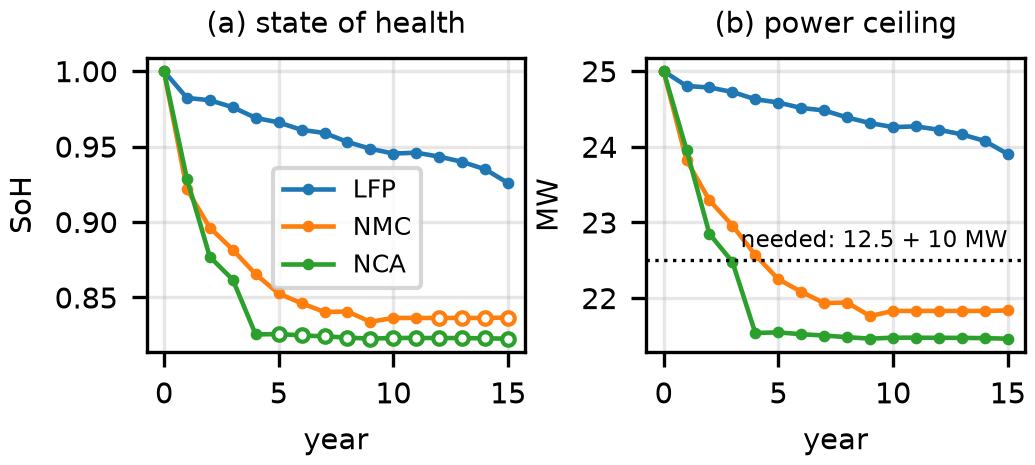
\includegraphics[width=\columnwidth]{fig_A.png}
\caption{(a) SoH from Model 1 and (b) power ceiling from Model 2 for the solar duty (wind within 0.01 SoH). Open markers: beyond the Sandia test length, held flat.}
\label{fig:A}
\end{figure}

\textbf{Within its limit an aged battery responds like a fresh one; past it, frequency is lost.} Inertia and droop are control settings, so they do not change with SoH. In Fig.~\ref{fig:B} the fresh, LFP and SoH-aware NCA batteries dip to 49.81\,Hz within 0.4\,s and recover to 49.97\,Hz. In the same hour an aged NCA battery run SoH-unaware hits its limit, crosses 49.4\,Hz in under 1\,s and settles at 48.7\,Hz (wind) with no recovery. Over all hours the simulation reproduces the hourly coverage test exactly (NCA wind: limit hit in 1.24\% of hours, 0.97\% below 49.4\,Hz).

\begin{figure}[t]
\centering
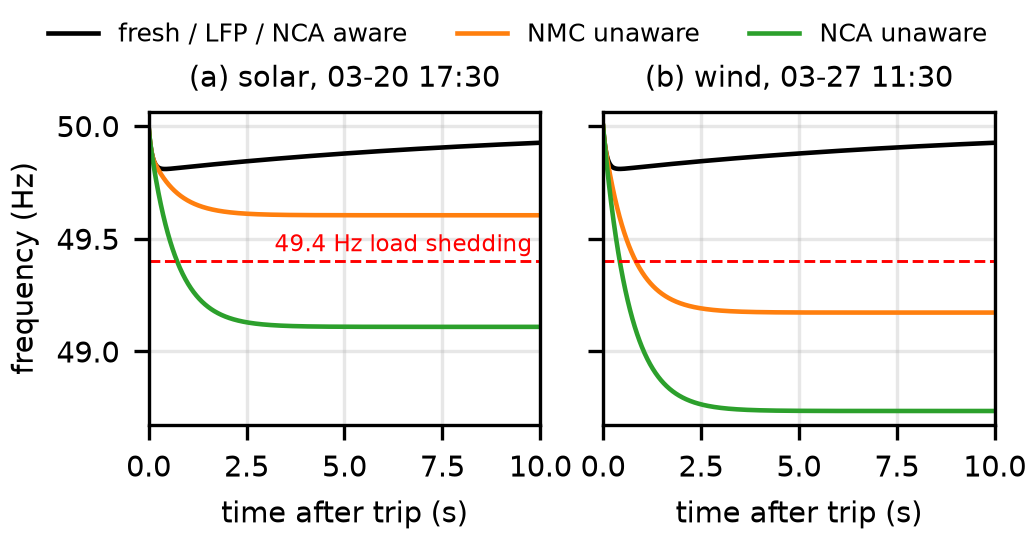
\includegraphics[width=\columnwidth]{fig_B.png}
\caption{Frequency after a 10\,MW trip at two real hours where the aged NCA battery falls short (year 10).}
\label{fig:B}
\end{figure}

\textbf{How often it happens, and the SoH-aware fix.} Fig.~\ref{fig:C} and Table~\ref{tab:res} give the share of trip hours the aged battery cannot cover. LFP covers every hour for 15 years. NCA starts failing in year 3 and NMC in year 5, reaching 0.6 / 0.5\% of hours for solar and 1.2 / 1.1\% for wind. Wind is about twice as exposed: it produces in twice as many hours and its battery is more often already discharging when a trip occurs. SoH-aware operation removes every failure, giving up no smoothing for solar and at most 0.15\% of the energy shifted for wind.

\begin{figure}[t]
\centering
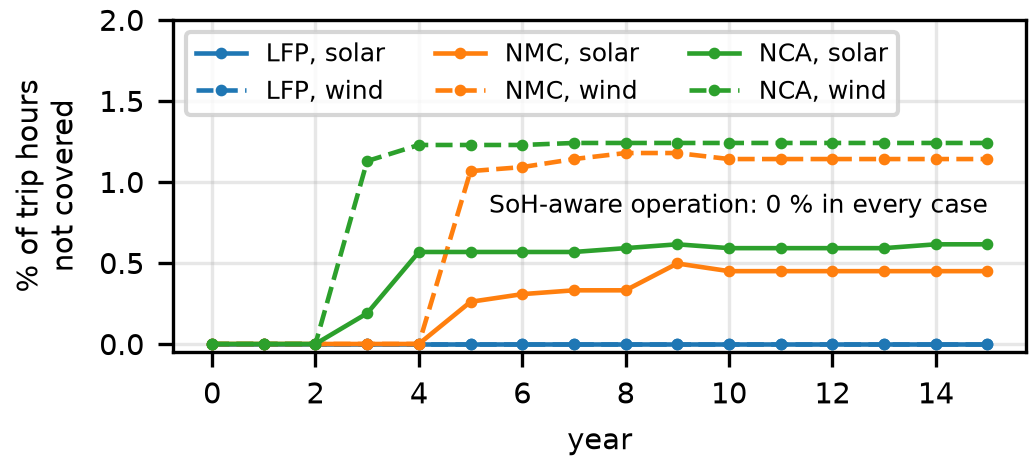
\includegraphics[width=\columnwidth]{fig_C.png}
\caption{Share of hours in which the aged battery cannot cover a 10\,MW trip, SoH-unaware operation.}
\label{fig:C}
\end{figure}

\begin{table}[t]
\centering
\caption{Year-10 results (solar / wind)}
\label{tab:res}
\begin{tabular}{lccc}
\toprule
 & LFP & NMC & NCA \\
\midrule
SoH & 0.95 & 0.84 & 0.82 \\
Power ceiling (MW) & 24.3 & 21.8 & 21.5 \\
Trips not covered, unaware (\%) & 0 / 0 & 0.45 / 1.14 & 0.59 / 1.24 \\
Below 49.4\,Hz, unaware (\%) & 0 / 0 & 0.26 / 0.64 & 0.45 / 0.97 \\
Trips not covered, SoH-aware (\%) & 0 / 0 & 0 / 0 & 0 / 0 \\
Extra rating for 25\,MW at year 15 & +5\% & +15\% & +17\% \\
\bottomrule
\end{tabular}
\end{table}

\textbf{Sizing.} Without SoH-aware operation the rating must cover the resistance rise: about 5\% extra for LFP and 15 to 17\% for NMC and NCA (Table~\ref{tab:res}). A sweep of 24 sizes (15 to 35\,MW, 1 to 4\,h) shows that the power reserve matters most, while extra energy does not help: a 4\,h battery is more often discharging at its limit.

\section{Conclusion and Future Scope}
In a solar-only or wind-only system, an ageing grid-forming battery delivers the same synthetic inertia response as a new one until its power ceiling falls below what it is asked to carry; then it loses control of frequency. LFP stays clear of that point for 15 years, while NMC and NCA cross it after 3 to 5 years, with wind exposed about twice as often as solar. Tracking SoH with the trained models and protecting the reserve removes the problem at almost no cost; otherwise the power reserve, not the energy, should be oversized.

Future work: (i) resistance data for NMC and NCA, to replace the LFP-based curve used for all chemistries here; (ii) grid-scale cells and longer tests, as Sandia's tests end after about 4 (NCA) and 11 (NMC) years of this duty; (iii) measured demand from a real isolated system, in place of load set equal to supply; (iv) validation of the frequency response against field events or a detailed inverter model; (v) real-time SoH-aware control fed by battery management data.

\begin{thebibliography}{4}
\bibitem{preger2020} Y. Preger \emph{et al.}, ``Degradation of commercial lithium-ion cells as a function of chemistry and cycling conditions,'' \emph{J. Electrochem. Soc.}, vol. 167, 120532, 2020.
\bibitem{severson2019} K. A. Severson \emph{et al.}, ``Data-driven prediction of battery cycle life before capacity degradation,'' \emph{Nature Energy}, vol. 4, pp. 383--391, 2019.
\bibitem{staffell2016} I. Staffell and S. Pfenninger, ``Using bias-corrected reanalysis to simulate current and future wind power output,'' \emph{Energy}, vol. 114, pp. 1224--1239, 2016.
\end{thebibliography}

\end{document}
